\documentclass[problem]{mcs}

%%%%%%%%%%%%%%%%%%%%%%%%%%%%%%%%%%%%%%%%%%%%%%%%%%%%%%%%%%%%%%%%%%%%%
% Problem starts here
%%%%%%%%%%%%%%%%%%%%%%%%%%%%%%%%%%%%%%%%%%%%%%%%%%%%%%%%%%%%%%%%%%%%%

% S09

\begin{problem}
Two nonparallel lines in the real plane intersect at a point.
Algebraically, this means that the equations
\begin{align*}
y & =  m_1 x + b_1 \\
y & =  m_2 x + b_2
\end{align*}
have a unique solution $(x, y)$, provided $m_1 \neq m_2$.  This statement
would be false if we restricted $x$ and $y$ to the integers, since the two
lines could cross at a noninteger point:

\centerline{\resizebox{!}{1in}{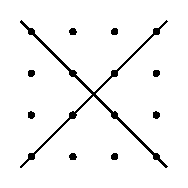
\includegraphics{figures/integerlines}}}

However, an analogous statement holds if we work over the integers
\emph{modulo a prime}, $p$.  Find a solution to the congruences
\begin{align*}
y & \equiv  m_1 x + b_1 \pmod{p} \\
y & \equiv  m_2 x + b_2 \pmod{p}
\end{align*}
when $m_1 \not\equiv m_2 \pmod{p}$.  Express your solution in the form $x
\equiv ? \pmod{p}$ and $y \equiv ? \pmod{p}$ where the ?'s denote
expressions involving $m_1$, $m_2$, $b_1$, and $b_2$.  You may find it
helpful to solve the original equations over the reals first.

\solution{Subtracting the second congruence from the first, we have:
\begin{eqnarray*}
0 & \equiv & m_1 x+b_1 - (m_2 x + b_2)  \pmod{p} \\
(m_1 - m_2)x & \equiv & b_2 - b_1 \pmod{p} \\
x & \equiv & (m_1 - m_2)^{-1} \cdot (b_2 - b_1) \pmod{p}
\end{eqnarray*}
Substituting this value of $x$ into the first congruence, we have
\[
y  \equiv  m_1 \cdot (m_1 - m_2)^{-1} \cdot (b_2 - b_1) + b_1 \pmod{p}
\]
Here $(m_1 - m_2)^{-1} \pmod p$ exists because $m_1 \not\equiv m_2
\pmod{p}$ and hence $p$ does not divide $(m_1 - m_2)$.

\textbf{Further exercise:} Show that $(x,y)$ are unique modulo $p$.
}

\end{problem}

%%%%%%%%%%%%%%%%%%%%%%%%%%%%%%%%%%%%%%%%%%%%%%%%%%%%%%%%%%%%%%%%%%%%%
% Problem ends here
%%%%%%%%%%%%%%%%%%%%%%%%%%%%%%%%%%%%%%%%%%%%%%%%%%%%%%%%%%%%%%%%%%%%%

\endinput
